\section{Methods}
\label{sec:methods}

\subsection{Related work}

There are already existing APIs or tools to download, inference and train AI
models:
\begin{itemize}
  \item Transformers (Hugging Face API) \cite{wolf-etal-2020-transformers}
  \item Cellpose API \cite{Stringer2020.02.02.931238}
  \item BioImage.IO Core (Python libraries)
  \item SAM2 repository \cite{ravi2024sam2}
\end{itemize}

The problem is there are no common APIs/CLIs/no standard.

For example with 'download API', there are 4 differents code for these 4 repositories:

\begin{listing}[H]
  \begin{minted}[frame=lines,framesep=2mm,baselinestretch=0.8,fontsize=\footnotesize,linenos]{python}
    # BioImage.IO
    model = load_description(args.model)

    # Hugging Face
    pipe = pipeline(task="mask-generation",
      model=args.model, points_per_batch=32,
      device=device)

    # SAM2
    mask_generator = SAM2AutomaticMaskGenerator
      .from_pretrained(args.model, device=device)
  \end{minted}

  \begin{minted}[frame=lines,framesep=2mm,baselinestretch=0.8,fontsize=\footnotesize,linenos]{bash}
    # Cellpose
    python -m cellpose --pretrained_model cyto3
  \end{minted}
\end{listing}

There is the same issue with 'inference API', 'train API', etc.

\subsection{Our approach}

We use existing APIs of AI repositories and use them in the context of WIPP. We
use AI model card to document AI model trained in WIPP.

Our contributions are:
\begin{itemize}
  \item Analyze API of AI repositories
  \item Implement them for containerized plugin that run in WIPP without learning the API
  \item Trained/Retrained AI model will comes with proper AI model card
\end{itemize}

\subsection{Web Image Processing Pipelines}

WIPP is a scientific workflow engine, illustrated as shown in figure 1.
The purpose of this tool is to make measurements based on terabyte-sized images.
It is an algorithmic plugin platform. Its goal is to lower the bar to execute
image analyses.

\begin{figure}[H]
  \centering
  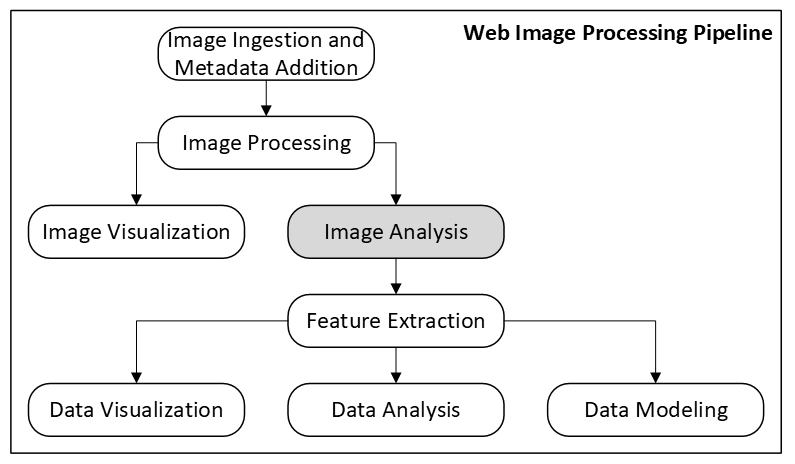
\includegraphics[width=1.0\linewidth]{png/methods/wipp.png}
  \caption{\Gls{WIPP}}
  \label{fig:1wipp}
\end{figure}

WIPP worflows are sequence of plugins. WIPP plugins are piece of code (code put
in the form of a container) taking inputs and outputs and executing code.

Thanks to a plugin you can, for example, load an \Gls{AiModel} hosted in
\Gls{WIPP}, specify an
image collection and perform the \Gls{AiInference} of this \Gls{AiModel} on the
selected images.
The result will be a new collection of images modified by the \Gls{AiModel}, for
example
with a label after inference of a \Gls{ClassificationModel}.

\subsection{Access public \Gls{AiRepositories}}

There are many public AI models on lots of public AI repositories.

\begin{table}[H]
  \centering
  \caption{Number of models per repository}
  \begin{tabular}{lcc}
    \toprule
    AI repositories & IC models & S + MG models \\
    \midrule
    Hugging Face    & 15,593                      & 1,160 + 176 \\
    BioImage.IO     & 1                           & 4 + 32 \\
    Cellpose        & $\times$                    & 21 \\
    SAM2            & $\times$                    & 8 \\
    PyTorch Hub     & 20                          & 5 \\
    \bottomrule
  \end{tabular}
  \caption*{Image Classif. (IC), Segmentation (S), Mask Generation (MG)}
\end{table}

Our goal is to access external AI models in WIPP.


We have developed new inference plugins, see figure 2, to enable access to
\Gls{AiModel}s available on different public \Gls{AiRepositories} such as
Hugging Face, BioImage.IO, Cellpose, and more.

\begin{figure}[H]
  \centering
  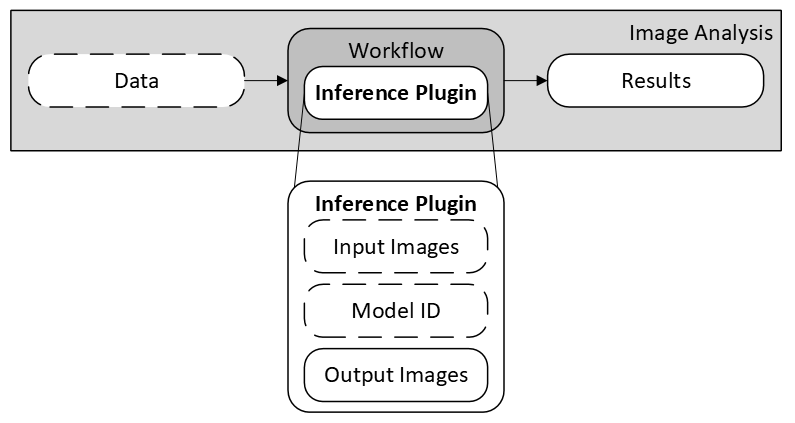
\includegraphics[width=1.0\linewidth]{png/methods/inference_plugin.png}
  \caption{Inference Plugin}
  \label{fig:2inference}
\end{figure}

This was achieved by developing general-purpose code using the \Gls{API} of
the various platforms. This
enabled us to increase the number of \Gls{AiModel}s usable
in \Gls{WIPP} thanks to containerized software.

\subsection{Document \Gls{AiModel}s}

We have introduced \Gls{AiModelCard} entries that are necessary for matching tasks
with \Gls{AiModel}s. This information will also be needed as runtime parameters.
Figure 3, training an \Gls{AI} in \Gls{WIPP} automatically generates its documentation
(\Gls{AiModelCard}).

\begin{figure}[H]
  \centering
  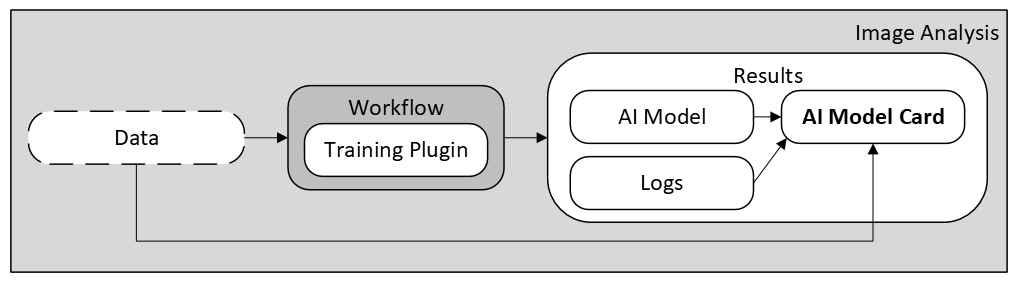
\includegraphics[width=1.0\linewidth]{png/methods/ai_model_card.png}
  \caption{\Gls{AiModelCard}}
  \label{fig:3aimodelcard}
\end{figure}

This was achieved by developing code to retrieve information about the \Gls{AiModel}
throughout the pipeline: name, creation date, data used for training, number of
iterations, training time, and more.

\subsection{Compute accuracy}

Our goal is to mesure accuracy of external AI results and to select the most
accurate/fastest one.

We have developed a new plugin, see figure 4, to compute the \Gls{DiceIndex}.

The formula is:

\[ Dice = \frac{2*TP}{2*TP + FP + FN} \]

It is a statistic used to gauge the similarity of two samples, in
our case images.

\begin{figure}[H]
  \centering
  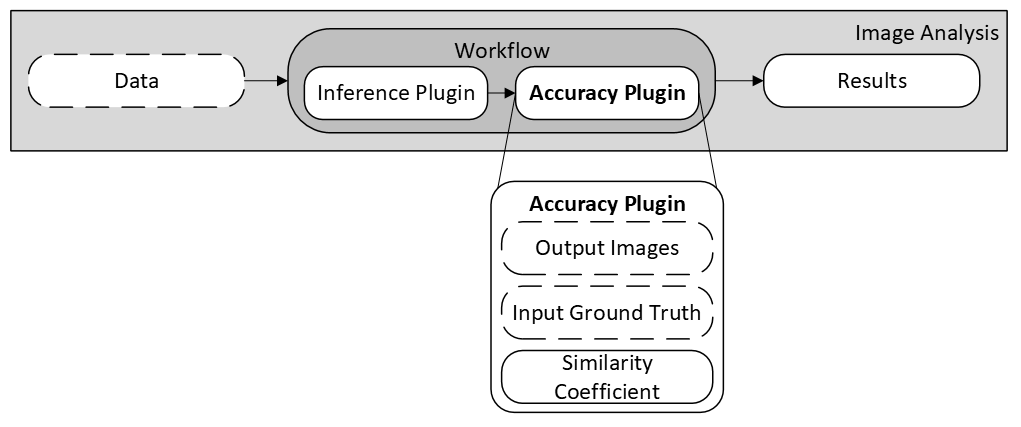
\includegraphics[width=1.0\linewidth]{png/methods/accuracy.png}
  \caption{Accuracy Plugin}
  \label{fig:4accuracy}
\end{figure}

This was achieved by implementing the \Gls{DiceIndex}'s formula into a containerized
software (plugin). This makes it now possible to sequence model \Gls{AiInference} (a
model created within \Gls{WIPP} or a model from a repository) and evaluate the
accuracy of the result provided, by comparing it with
\Gls{GroundTruthData}.
